\documentclass{article}
\usepackage[utf8]{inputenc}
\usepackage{amsmath}
\usepackage{amstext}
\usepackage{graphicx}
\usepackage{esint}
\usepackage{geometry}
\usepackage{hyperref}
\usepackage{amsfonts}

\hypersetup{
    colorlinks=true,
    linkcolor=blue,
    filecolor=magenta,      
    urlcolor=cyan,
    pdftitle={Overleaf Example},
    pdfpagemode=FullScreen,
    }
\geometry{verbose,lmargin=2cm,rmargin=2cm}

\title{Autoregressive neural network of spins system: the deepness of Mean-Field models}
%\author{indaco biazzo and ...}
\date{June 2022}

\begin{document}

\maketitle

\tableofcontents

\section{Introduction}

\section{Materials and Methods}
\subsection{Pair-wise Ising model in autoregressive conditional probability form}
Consider a generic Hamiltonian $H[\underline{x}]$ that depends on a set $N$ of binary variable $\underline{x}$. The Boltzmann distribution at inverse temperature $\beta$ is:
\begin{equation}
P\left(\mathbf{x}\right)=\frac{e^{-\beta H\left(\mathbf{x}\right)}}{\sum_{\left\{ x\right\} }e^{-\beta H\left(\mathbf{x}\right)}}.
\end{equation}
In general it is difficult to compute marginals and to average quantities when $N$ is large, and on several systems sampling from this distributions is difficult. If we are able to rewrite the Boltzmann distribution in autoregressive form:
\begin{equation}
P\left(\mathbf{x}\right)=\prod_{i}P\left(x_{i}|\mathbf{x}_{<i}\right)
\end{equation}
then it would be very easy to produce independent samples from it thanks to the ancestral sampling procedure. It has been proposed to use a variational approach to approximate the Boltzmann distribution with a trial probability distribution that has this autoregressive form and each conditional probability is represented by a feed forward neural network with set a of parameters ${\theta}$:
\begin{equation}
Q^{\theta}\left(\mathbf{x}\right)=\prod_{i}Q^{\theta_i}\left(x_{i}|\mathbf{x}_{<i}\right)
\end{equation}
The parameters ${\theta}$ can be learn minimizing the Kullback-Liebler divergence $D_{KL}$,
with the true probability function:

\begin{eqnarray*}
D_{KL}\left(P|Q^{\Theta}\right) & = & \sum_{\left\{ x\right\} }Q^{\Theta}\left(\left\{ x\right\} \right)\ln\left(\frac{Q^{\Theta}\left(\left\{ x\right\} \right)}{P\left(\left\{ x\right\} \right)}\right)\\
 & \approx & \sum_{x\sim Q^{\Theta}}\left[\ln\left(Q^{\Theta}\left(\left\{ x\right\} \right)\right)-\ln\left(P\left(\left\{ x\right\} \right)\right)\right]
\end{eqnarray*}
where we substituted the sum over all $\{x\}$ configurations with a set of configurations extracted, thanks to the ancestral sampling, from the autoregressive trial functions.
Up to here the approach seems clear. 
What is less clear, is what architecture of the neural networks we have to use for each problem.
There is a large number of systems where the analytic form of the Boltzmann distribution is known, at least in some limits (for instance $N\rightarrow \infty$). 
In this work we want to find neural network architectures that could precisely represent solvable statistical physics systems. 
Then, these architectures could be used as an ansatz for more complex systems or in different limits (for instance at finite $N$).


\subsubsection{Conditionals}
The autoregressive probability distribution has this form:
\begin{equation}
P\left(\mathbf{x}\right)=\prod_{i}P\left(x_{i}|\mathbf{x}_{<i}\right)
\end{equation}
where the $\mathbf{x}_{<i}=\left(x_{1},x_{2}\dots x_{i-1}\right)$
are the spins with index lower than $i$. We want to find a form of a generic $i$ conditional probability: 

\begin{eqnarray}
P\left(x_{i}|\mathbf{x}_{<i}\right) & = & \frac{\sum_{x_{i+1}\dots x_{N}}e^{-\beta H}}{\sum_{x_{i}\dots x_{N}}e^{-\beta H}} = \frac{f\left(x_{i},\mathbf{x}_{<i}\right)}{\sum_{x_{i}}f\left(x_{i},\mathbf{x}_{<i}\right)}
\label{eq:chain}
\end{eqnarray}
as a feed forward neural network in known and solvable statistical physics systems. Without loss of generality we consider the conditional probability $P\left(x_{i}=1|\mathbf{x}_{<i}\right)$; we rewrite the term in the following way: 
\begin{eqnarray}
\label{eq:sigma_log}
P\left(x_{i}=1|\mathbf{x}_{<i}\right) & = & \frac{f\left(x_{i}=1,\mathbf{x}_{<i}\right)}{\sum_{x_{i}}f\left(x_{i},\mathbf{x}_{<i}\right)}\\
& = &\frac{f\left(x_{i}=1,\mathbf{x}_{<i}\right)}{f\left(x_{i}=1,\mathbf{x}_{<i}\right)+f\left(x_{i}=-1,\mathbf{x}_{<i}\right)}\\
& = &\frac{1}{1+\frac{f\left(x_{i}=-1,\mathbf{x}_{<i}\right)}{f\left(x_{i}=1,\mathbf{x}_{<i}\right)}} = \frac{1}{1+e^{\log\left(f\left(x_{i}=-1,\mathbf{x}_{<i}\right)\right)-\log\left(f\left(x_{i}=1,\mathbf{x}_{<i}\right)\right)}}\\
& = &\sigma\left(\log\left[f\left(x_{i}=1,\mathbf{x}_{<i}\right)\right]-\log\left[f\left(x_{i}=-1,\mathbf{x}_{<i}\right)\right]\right)
\end{eqnarray}

where $\sigma(x)=\frac{1}{1+e^{-x}}$. In this way the end of our feed-forward neural network is a sigma function that assure that the values is
between 0 and 1. The terms:
\begin{equation}
\log\left[f\left(x_{i}=\pm 1,\mathbf{x}_{<i}\right)\right] = \log \left[ \sum_{x_{i+1}\dots x_{N}}e^{-\beta H}\delta_{x_i, \pm1} \right] 
\end{equation}
are very close to the usual free entropy computed in statistical physics.
We consider a generic fully connected two body interaction Hamiltonian of binary spin variables:
\begin{equation}
    H = -\sum_{i<j} J_{ij} x_i x_j - \sum_{i} h_i x_i
\end{equation}
Considering a generic variable $i$, we rewrite the Hamiltonian splitting the contributions that come from variables with index smaller and larger than $i$, labelled, respectively, $s$ and $l$ :
\begin{equation}
    H = H_{ss} + H_{si} + H_{il} + H_{sl} + H_{ll}
\end{equation}
We have defined:
\begin{eqnarray}
    H_{ss} & = & - \sum_{s=1}^{i-1}\sum_{s'=s+1}^{i-1} J_{ss'} x_s x_{s'} - \sum_{s} h_s x_s \\
    H_{si}[x_i = \pm 1] & = & \mp \left(h_i + \sum_{s=1}^{i-1} J_{si} x_s\right)\\
    H_{il}[x_i = \pm 1] & = & \mp \sum_{l=i+1}^{N} J_{il} x_l \\
    H_{sl} & = & - \sum_{l=i+1}^{N}\sum_{s=1}^{i-1} J_{sl} x_s x_l\\
    H_{ll} & = & - \sum_{l=i+1}^{N}\sum_{l'=l+1}^{N} J_{ll'} x_l x_{l'} + \sum_{l=i+1}^N h_l x_l\\
\end{eqnarray}
Substituting tho above terms, of a generic two body interaction Hamiltonian, in eq.\ref{eq:sigma_log} we obtain:
\begin{equation}
P\left(x_{i}=1|\mathbf{x}_{<i}\right) = \sigma\left( 
 2 \beta H_{si}[x_i = +1] +\log(\rho_i^+) - \log(\rho_i^-)
\right),
\end{equation}
where:
\begin{eqnarray}
\rho_i^{\pm}[\mathbf{x}_{<i}] &=& \sum_{x_{i+1}\dots x_{N}} e^{-\beta \left(
H_{li}[x_i = \pm 1] + H_{sl} + H_{ll}\right)} \\
& = & \sum_{x_{i+1}\dots x_{N}} \exp\left\{
\beta\sum_{l=i+1}^{N}\left( \pm J_{il} + \sum_{s=1}^{i-1} J_{sl} x_s + h_l \right) x_l + \beta\sum_{l=i+1}^{N}\sum_{l'=l+1}^{N} J_{ll'} x_l x_{l'}
\right\}
\end{eqnarray}
The terms $H_{qq}$ cancel out.
The computational cost of the sum over all the configuration of spins labelled with $l$ grows exponentially with the systems size making it unfeasible after a few number of spins the explicit computations. The idea is to find feed-forward neural network architectures representing these functions with a polynomial number of free parameters.   
In the following we will explore, on known and solvable statistical physic systems, if it is possible to find neural network architectures or functional forms to compact represent (not exponentially in N) this conditional probability. We start considering the Curie-Weiss model, then moving to more complex systems, the random field Ising model and Sherrington–Kirkpatrick model.

\subsection{Models}
\subsubsection{Curie-Weiss model}

The Curie-Weiss model is a uniform fully-connected Ising model. Its Hamiltonian, with $N$ spins, is:

\begin{equation}
H\left(\mathbf{x}\right)=-h\sum_{i=1}^{N}x_{i}-\frac{J}{N}\sum_{i<j}x_{i}x_{j}
\doteq -h\sum_{i=1}^{N} S - \frac{J}{2N}S^2 - \frac{J}{2}
\end{equation}
 where we have defined $S=\sum_{i=1}^{N}x_{i}$.\\
 The conditional probability of a spin $i$ to be up, given the configuration of the other smaller spins $s$:
\begin{equation}
P\left(x_{i}=1|\mathbf{x}_{<i}\right) = \sigma\left( 
 2 \beta h + 2 \beta \frac{J}{N}\sum_{s=1}^{i-1}x_s +\log(\rho_i^+[\mathbf{x}_{<i}]) - \log(\rho_i^-[\mathbf{x}_{<i}])
\right),
\end{equation}
where:
\begin{equation*}
\rho_i^{\pm}[\mathbf{x}_{<i}] = \sum_{x_{i+1}\dots 
x_{N}}e^{\beta \left(h\pm\frac{J}{N}+\frac{J}{N}\sum_{s=1}^{i-1}x_{s}\right)S_{i}+\frac{\beta J}{2N}S_{i}^{2}} = 
\sum_{x_{i+1}\dots x_{N}} e^{\beta h_i^{\pm}[\mathbf{x}_{<i}]S_i +\frac{\beta J}{2N}S_{i}^{2}},
\end{equation*}
and we defined $h_i^{\pm}[\mathbf{x}_{<i}] = h\pm\frac{J}{N}+\frac{J}{N}\sum_{s=1}^{i-1}x_{s}$ and $S_i=\sum_{l=i+1}^{N}x_{l}$. The sums over the configurations of the spins $l$ can be carried on easily:
\begin{eqnarray*}
 \rho_i^{\pm}[\mathbf{x}_{<i}] & = & \sum_{x_{i+1}\dots x_{N}} e^{\beta h_i^{\pm}[\mathbf{x}_{<i}]S_i +\frac{\beta J}{2N}S_{i}^{2}}
  = \sqrt{\frac{N}{2\pi \beta J}}\sum_{x_{i+1}\dots x_{N}}e^{\beta h_i^{\pm}[\mathbf{x}_{<i}] S_{i}}\int e^{-\frac{N}{2J \beta}t^{2}+t S_{i}} dt\\
 & = & \sqrt{\frac{N}{2\pi \beta J}}\int dt e^{-\frac{N}{2J \beta}t^{2}} \sum_{x_{i+1}\dots x_{N}}e^{(\beta h_i^{\pm}[\mathbf{x}_{<i}] + t) S_{i}}  
 =  \sqrt{\frac{N}{2\pi \beta J}}\int dt e^{-\frac{N}{2J \beta}t^{2}} \left(e^{\beta h_i^{\pm}[\mathbf{x}_{<i}] + t} + e^{ (-\beta h_i^{\pm}[\mathbf{x}_{<i}] - t)} \right)^{N-i}  \\ 
 \label{eq:rho_last_exact}
 \end{eqnarray*}
 whwre we used the Hubbard–Stratonovich (HS) transformation to get the second equality.\\
 First, in the following,  we derive the exact expression of the this conditional probability and how it can be expressed as a feed forward neural network, then the limit to $n\rightarrow N$ we derive a new architecture with smaller number of parameters.\\


 \subsubsection{Exact expression of the conditional probability of the Curie-Weiss model}
 The integral in the equation \ref{eq:rho_last_exact} can be computed the following way :

 \begin{eqnarray*}
 \rho_i^{\pm}[\mathbf{x}_{<i}] &=& \sqrt{\frac{N}{2\pi \beta J}}\int dt e^{-\frac{N}{2J \beta}t^{2}} 
 \sum_{k=0}^{N-i} \binom{N-i}{k} e^{(N-i-2k)*(\beta h_i^{\pm}[\mathbf{x}_{<i}] + t)}\\
 &=& \sum_{k=0}^{N-i} \binom{N-i}{k} \sqrt{\frac{N}{2\pi \beta J}}\int dt e^{-\frac{N}{2J \beta}t^{2}} 
  e^{(N-i-2k)*(\beta h_i^{\pm}[\mathbf{x}_{<i}] + t)}\\
&=& \sum_{k=0}^{N-i} \binom{N-i}{k}e^{\frac{\beta J}{2N}\left(N-i-2k\right)^{2}+\left(N-i-2k\right)\left(\beta h \pm \frac{\beta J}{N}\right)} e^{\frac{\beta J}{N}\left(N-i-2k\right) \sum_s x_s} \\
&=& \sum_{k=0}^{N-i} e^{a_{i,k}^{\pm} + b_{i,k}^{\pm} \sum_s x_s} 
\end{eqnarray*}
where we defined:
\begin{eqnarray}
\label{eq:params}
e^{b_{i,k}^{\pm}} & = & \binom{N-i}{k}e^{\frac{\beta J}{2N}\left(N-i-2k\right)^{2}+\left(N-i-2k\right)\left(\beta h \pm \frac{\beta J}{N}\right)}\\
e^{\omega_{i,k}^{\pm}} & = & e^{\frac{\beta J}{N}\left(N-i-2k\right)}.
\end{eqnarray}
The the final feed-forward architecture of the neural network is:
\begin{eqnarray}\
\label{eq:curie_weiss_cond}
Q^{\Theta}\left(x_{i}=+1|\mathbf{x}_{<i}\right) & = &  \sigma \left(b_{i}+\omega_{i}\sum_{s=1}^{i-1}x_{s}-\log\left[\sum_{k=0}^{N-i}e^{b_{i,k}^{+}+w_{i,k}^{+}\sum_{s=1}^{i-1}x_{s}}\right]+\log\left[\sum_{k=0}^{N-i}e^{b_{i,k}^{-} + w_{i,k}^{-}\sum_{s=1}^{i-1}x_{s}}\right]\right).
\end{eqnarray}
where $b_i=2\beta h$ and $\omega_i=\frac{2\beta J}{N}$. 
\newline
This function can be interpreted as a feed-forward neural network; see fig.\ref{fig:curie_weiss}. 
The parameters of this neural network have an analytic dependence from the parameters $J$ and $h$ of the Boltzmann distributions. 
The set of parameters ($b_i, b_i^{k\pm}, \omega_i, \omega_i^{k\pm}$) can be consider as free parameters trained to minimize the KL divergence with the true probability distribution. 
It is interesting to note the number of parameters of each conditional probability distribution $i$ are $2+4(N-i)$; they decrease as $i$ increase as well as their number of variable in the input. This results is, somehow, the opposite on what usually the architecture should take care, meaning enlarging the number of input variables the number of parameters should increase as well to describe the complexity of the function to represent. Moreover the conditional probability neural network depends only of the sum of the input variables.
The total number of parameters of all conditional probability distribution scale as $O(N^2)$. 

\begin{figure}[!h]
    \centering
    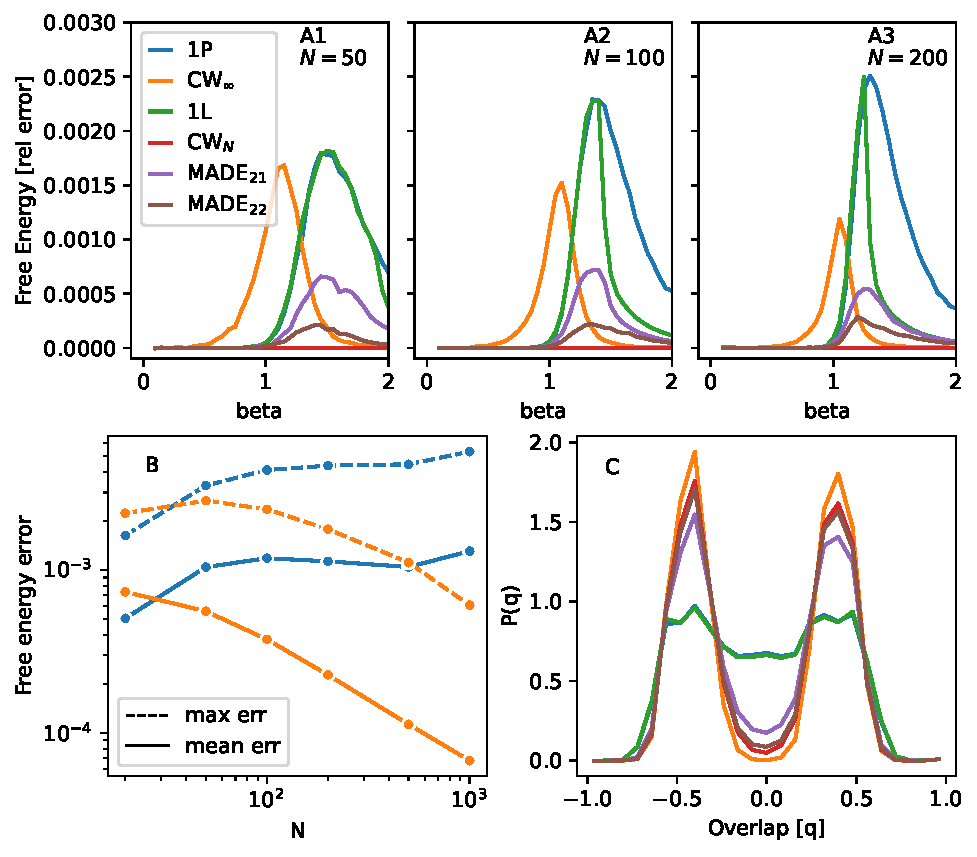
\includegraphics[width=1\textwidth]{img/CW_res.pdf}
    \caption{Results}
    \label{fig:curie_weiss}
\end{figure}


\subsubsection{Saddle point method}
Now we derive a new neural network architecture in the limit of $N \gg 1$. For simplicity the $h=0$ case is considered. Introducing the following variables: $\rho_i = \frac{N-i}{N}$, $m_i = -\frac{N-i-2k}{N}$, we can write:
 \begin{align*}
 \rho_i^{\pm}[\mathbf{x}_{<i}] &= \sqrt{\frac{N}{2\pi \beta J}}\int dt e^{-\frac{N}{2J \beta}t^{2}} 
 \sum_{k=0}^{N-i} \binom{N-i}{k} e^{(N-i-2k)*(\beta h_i^{\pm}[\mathbf{x}_{<i}] + t)}\\
 &= \sum_{k=0}^{N-i} \binom{N-i}{k}e^{\frac{\beta J}{2N}\left(N-i-2k\right)^{2}+\left(N-i-2k\right)\left(\pm\frac{\beta J}{N}\right)} e^{\frac{\beta J}{N}\left(N-i-2k\right) \sum_s x_s} \\
 &= \sum_{m_i=-\rho_i}^{\rho_i} \binom{N\rho_i}{\frac{N(m_i+\rho_i)}{2}} e^{\frac{N \beta J}{2}m_i^{2} \mp \beta J m_i } e^{N \rho_i \beta J \frac{\sum_s x_s}{N-i}}
\end{align*}
In the limit $N \gg 1$, and using the Stirling approximation for the binomial factor we obtain:
 \begin{align*}
 \rho_i^{\pm} &= 
  \int_{-\rho_i}^{\rho_i} \binom{N\rho_i}{\frac{N(m_i+\rho_i)}{2}} e^{\frac{N \beta J}{2}m_i^{2} \mp \beta J m_i } e^{N \rho_i \beta J \frac{\sum_s x_s}{N-i}} dm_i \\
& =  \int_{-\rho_i}^{\rho_i} \exp\left\{-N\rho\left( -\frac{1+\frac{m_i}{\rho_i}}{2} \log\frac{1+\frac{m_i}{\rho_i}}{2} - \frac{1-\frac{m_i}{\rho_i}}{2} \log\frac{1-\frac{m_i}{\rho_i}}{2}   - \frac{\beta m_i^2}{2 \rho_i} + \beta m_i \frac{\sum_s x_s}{N-i}\right) \right\} e^{\mp \beta J m_i}
\end{align*}
Now we use the saddle point method to evaluate this integrals, computing the extremes of the function inside the curly brackets. Deriving by $m_i$ we obtain that the extremes should satisfy the following equation:
\begin{equation}
\frac{m_i}{\rho_i} = \tanh \left( \beta(\frac{m_i}{\rho_i} - \frac{\sum_s x_s}{N-i}) \right)
\label{eq:extrem_i}
\end{equation}
In the $N$ large limit, and for a typical sample, we assume that: $\frac{\sum_s x_s}{N-i} \approx |\tilde{m}_{\beta}| \text{sign}(\sum_s x_s)$, where the $\tilde{m}_{\beta}$ is the magnetization of the Curie-Weiss system at inverse temperature $\beta$ and $\text{sign(x)} = \frac{|x|}{x}$ is the sign function.
We can distinguish two cases when the magnetization of the system is zero or different from zero. 
In the first case, when $\beta\leq1$, the solution of eq.\ref{eq:extrem_i} is zero as well, and $\log(\rho_i^{+}) - \log(\rho_i^{-})=0$ because the only term that depends on the sign, $\mp \beta J m_i$, vanish.\\ 
When instead the system acquire a magnetization $\tilde{m}_{\beta}$ different from zero, the eq.\ref{eq:extrem_i} admit one maximum, that depends on the two possible symmetric values of $\frac{\sum_s x_s}{N-i}\approx |\tilde{m}_{\beta}| \text{sign}(\sum_q x_q)$. 
The solution of eq.\ref{eq:extrem_i}, $\pm \tilde{m}_{\text{extrem}}$ depends again on $\text{sign}(\sum_s x_s)$. 
Once again we can write the maximum solution as $\tilde{m}_{i}=|\tilde{m}_i| \text{sign}(\sum_s x_s)$. 
Easily we obtain that $\log(\rho_i^{+}) - \log(\rho_i^{-}) = -2\beta J|\tilde{m}_i| \text{sign}(\sum_s x_s)$. 
We can use a trial function in this form:
\begin{eqnarray}\
\label{eq:curie_weiss_cond2}
Q^{\Theta}\left(x_{i}=+1|\mathbf{x}_{<i}\right) & = & \text{sigma}\left(\omega_{i}^0\sum_{s=1}^{i-1}x_{s} + \omega_i^1 \text{sign}(\sum_{s=1}^{i-1}x_{s})\right).
\end{eqnarray}
where $\omega_i^{1,2}$ are free parameters to be trained. The number of parameters in this case scale as $O(N)$.

\section{spin glass}
Consider the hamiltonian of a spin glass with zero external field for simplicity:
\begin{equation}
H\left(\mathbf{x}\right)=-\sum_{i<j}J_{ij}x_{i}x_{j}
\end{equation}
where the set of $\underline{J}$ are i.i.d. random variable extracted from a Gaussian probability distribution $P(J)=\sqrt{\frac{N}{2\pi}}\exp\left(\frac{-NJ^2}{2} \right)$. \\
To find a feed-forward representation of the conditional probability of the Sherrington-Kirkpatrick model we use the replica trick \cite{}. We assume that $N-i$ is large enough such that the following approximation is valid for the partial partition function $\rho_i$: 
\[
\log\rho_i^{\pm} \sim \mathbb{E}\left[  \log\rho_i^{\pm} \right] = \lim_{n\rightarrow 0} \frac{  \log(\mathbb{E}\left[(\rho_i^{\pm})^n \right])}{n}
\]

Where in the last passage we use the replica trick. We assume that the quantity $\log\rho_i^{\pm}$ is a self-averaged quantity on the $N-i$ variables. The replica computation can be carried on easly, finding:
\begin{eqnarray}
\mathbb{E}_{\underline{J}}\left[(\rho_i^{\pm}[\mathbf{x}_{<i}])^n \right] & = & 
\int \prod_{l<l'} dP_{J_{ll'}} \left[ 
\sum_{\{\underline{x}^{a}\}_{i+1}^N} \exp\left\{\beta \left[
\sum_{l,a}\left( \pm J_{il} + \sum_{s} J_{sl} x_s \right) x_l^{a} + \sum_{l,l', a} J_{ll'} x_l^{a} x_{l'}^{a}
\right]  \right\} 
\right]\\
\end{eqnarray}
where, the sums over $(l,l')$, $s$ and $a$ run respectively over $(i+1,N)$, $(1,i-1)$ and $(1,n)$, and $dP_{J_{ll'}}=P(J_{ll'})dJ_{ll'}$. We defined $h_l^{\pm}[\mathbf{x}_{<i}] =\pm J_{il} + \sum_{s=1}^{i-1} J_{sl} x_s$ and carrying out the integrals over the disorder variables $\{P(J_{ll'})\}$ yields:
\begin{eqnarray}
\mathbb{E}_{\underline{J}}\left[(\rho_i^{\pm}[\mathbf{x}_{<i}])^n \right] & = & 
\sum_{\{\underline{x}^{a}\}_{i+1}^N} 
\exp\left\{\beta \left[
\sum_{l} h_l^{\pm}[\mathbf{x}_{<i}] \sum_{a} x_l^{a} +\frac{\beta}{2N} \sum_{l,l'} \sum_{a,b} x_l^{a} x_l^{b} x_{l'}^{a}x_{l'}^{b} \right]  \right\} \\
& = & e^{ \frac{(N-i) \beta^2}{4N}((N-i)n-n^2) } 
\sum_{\{\underline{x}^{a}\}_{i+1}^N} 
\exp\left\{\beta \left[
\sum_{l} h_l^{\pm}[\mathbf{x}_{<i}] \sum_{a} x_l^{a} +\frac{\beta}{2N} \sum_{a<b} \left( \sum_{l}  x_l^{a} x_l^{b} \right)^2 \right]  \right\}
\end{eqnarray}
Using the Hubbard-Stratonovich transformation of the quadratic terms we car write:
\begin{eqnarray}
\mathbb{E}_{\underline{J}}\left[(\rho_i^{\pm}[\mathbf{x}_{<i}])^n \right] & = & 
c(n,N,i)
\int \prod_{a<b} dQ_{ab} e^{-\frac{N}{2}\beta^2Q_{a,b}^2}
\sum_{\{\underline{x}^{a}\}_{i+1}^N} 
\exp\left\{\beta \left[
\sum_{l} h_l^{\pm}[\mathbf{x}_{<i}] \sum_{a} x_l^{a} +\beta \sum_{a<b} Q_{a,b} \sum_{l}  x_l^{a} x_l^{b} \right]  \right\} \\
& = & 
c(n,N,i)
\int \prod_{a<b} dQ_{ab} e^{-\frac{N}{2}\beta^2Q_{a,b}^2}
\prod_{l} \left[
\sum_{\{\underline{x}^{a}_l\}} 
\exp\left\{\beta \left[
h_l^{\pm}[\mathbf{x}_{<i}] \sum_{a} x_l^{a} +\beta \sum_{a<b} Q_{a,b}  x_l^{a} x_l^{b} \right]  \right\}
\right] \label{eq:before_ansaltz}
\end{eqnarray}
where we defined $c(n,N,i) = e^{ \frac{(N-i) \beta^2}{4N}((N-i)n-n^2) } \left(\frac{2\pi \beta^2}{N}\right)^{\frac{n(n-1)}{2}}$. The well know Parisi solutions of the SK model prescribe how to parametrize \cite{} the matrix of the overlaps $Q$. In the following we show how to obtain neural network architectures based on the the replica symmetric (RS) and k-replica symmetric broken symmetry (k-RSB) solutions.


\subsection{Replica Symmetric solution (RS)}
We assume that the overlap between the replicas symmetric under permutations, and the matrix of the overlaps between replicas is parametrize with only one variable $q$:
$$
Q_{a,b}=\begin{cases}
			0, & \text{if $a=b$}\\
            q, & \text{otherwise}
		 \end{cases}
$$
Considering this ansatz we obtain:
\begin{eqnarray}
\mathbb{E}_{\underline{J}}\left[(\rho_i^{\pm, sym}[\mathbf{x}_{<i}])^n \right] & = & 
c(n,N,i)
\int dq e^{-\frac{n(n-1)N}{4}\beta^2 q^2}
\prod_{l} \left[
\sum_{\{\underline{x}^{a}_l\}} 
\exp\left\{\beta \left[
h_l^{\pm}[\mathbf{x}_{<i}] \sum_{a} x_l^{a} +\beta q \sum_{a<b} x_l^{a} x_l^{b} \right]  \right\} 
\right] \\
& = &
c(n,N,i)
\int dq e^{-\frac{n(n-1)N}{4}\beta^2 q^2}
e^{-\frac{nN\beta^2 q}{2}}
\prod_{l} \left[
\sum_{\{\underline{x}^{a}_l\}} 
e^{\beta \left[
h_l^{\pm}[\mathbf{x}_{<i}] \sum_{a} x_l^{a} + \frac{\beta q}{2} \left(\sum_{a} x_l^{a} \right)^2 \right]} 
\right]\\
& = &
c'(n,N,i)
\int dq e^{-\frac{n(n-1)N}{4}\beta^2 q^2}
e^{-\frac{nN\beta^2 q}{2}}
\prod_{l} \left[\int \frac{dz_l}{\sqrt{2\pi q}} e^{-\frac{z_l^2}{q}}
\sum_{\{\underline{x}^{a}_l\}} 
e^{\beta \left(
h_l^{\pm}[\mathbf{x}_{<i}] +\beta z_l \right) \sum_{a} x_l^{a}} 
\right]\\
& = &
c'(n,N,i)
\int dq e^{-nN\left(\frac{(n-1)}{4}\beta^2 q^2 +\frac{\beta^2 q}{2}\right)}
\prod_{l} \left[\int \frac{dz_l}{\sqrt{2\pi q}} e^{-\frac{z_l^2}{q}}
2^n\cosh^n \left(\beta \left(
h_l^{\pm}[\mathbf{x}_{<i}] +\beta z_l \right)\right) 
\right].\\
\end{eqnarray}
Using the limit that $n\rightarrow 0$ we can write:
\begin{eqnarray}
\int \frac{dz_l}{\sqrt{2\pi q}} e^{-\frac{z_l^2}{q}}
2^n\cosh^n \left(\beta \left(
h_l^{\pm}[\mathbf{x}_{<i}] +\beta z_l \right)\right) = e^{n \int \frac{dz_l}{\sqrt{2\pi q}} e^{-\frac{z_l^2}{q}}
\log 2\cosh \left(\beta \left(
h_l^{\pm}[\mathbf{x}_{<i}] +\beta z_l \right)\right)}.
\label{eq:gauss_n0}
\end{eqnarray}
And in the end we have:
\begin{eqnarray}
\log (\rho_i^{\pm, sym}[\mathbf{x}_{<i}]) & = & 
\lim_{n\rightarrow 0} \frac{1}{n} \log \left( c'(n,N,i)
\int dq e^{-\frac{n(n-1)N}{4}\beta^2 q^2}
e^{-\frac{nN\beta^2 q}{2}}
e^{n \sum_l 
\int \frac{dz_l}{\sqrt{2\pi q}} e^{-\frac{z_l^2}{q}}
\log 2\cosh \left(\beta \left(
h_l^{\pm}[\mathbf{x}_{<i}] +\beta z_l \right)\right)
} 
\right)\\
& = &
\log(c''(N,i)) + 
\left( +\frac{N}{4}\beta^2 q^2_0 
-\frac{N\beta^2 q_0}{2}
+ \sum_l 
\int \frac{dz_l}{\sqrt{2\pi q_0}} e^{-\frac{z_l^2}{q_0}}
\log 2\cosh \left(\beta \left(
h_l^{\pm}[\mathbf{x}_{<i}] +\beta z_l \right)\right)
\right) \\
& \doteq &  
c(N,i, q_0) -
\sum_l 
\int \frac{dz_l}{\sqrt{2\pi q_0}} e^{-\frac{z_l^2}{q_0}}
\log \sigma \left(\beta \left(
2h_l^{\pm}[\mathbf{x}_{<i}] +2\beta z_l \right)\right)
 \\
\end{eqnarray}
In the second line we use the saddle point methods to evaluate the integral over $q$, assuming tha the single maximum value $q_0$ doesn't depend from the input values $\mathbf{x}_{<i}$ in the set of $h_l^{\pm}[\mathbf{x}_{<i}]$. It is a strong assumption to be verified {\it a posteriori} on the goodness of the neural network architectures performances. In the third lines we simplify values that are the same between $\log(\rho^+)$ and $\log(\rho^-)$.

% We can, after some manipulations, obtain a more neural network friendly function:
% \begin{eqnarray}
% \log (\rho_i^{\pm, sym} [\underline{x_l}])^n] & \approx & 
% \text{Extr}_q \left( +\frac{N}{4}\beta^2 q^2 
% -\frac{N\beta^2 q}{2}
% + \sum_l 
% \int dz_l e^{-z_l^2}
% \log \cosh \left(\beta \left(
% h_l +\beta \sqrt{q}z_l \right)\right)
% \right) 
% \end{eqnarray}
Now we consider the following approximation of the following Gaussian convolution:
\[
\int dz e^{-z^2}
\log \sigma \left(\beta \left(
h +\beta \sqrt{q}z \right)\right) \sim b_0 + w_0*\log \sigma(b_1 + w_1 h) 
\]
Where $(b_0, w_0, b_1,w_1)$ are free parameters to be determined. In SI \cite{} a numerical analysis of the correctness of this approximation is shown.  
Putting together all the pieces we can parameterize the conditional probability as:
\begin{eqnarray}
Q^{RS}\left(x_{i}=1|\mathbf{x}_{<i}\right) & = & \sigma\left( 
-2 \beta H_{s}[x_i = +1] +\log(\rho_i^+) - \log(\rho_i^-)
\right) \\
& = & b_0^i + w_0^i\sum_q J_{si} x_{si} + \sum_{t \in \{+,-\}} w_0^{i,t} \sum_l \log\sigma(b_1^{i,t} + w_1^{i,t}\sum_{s} J_{sl} x_s) 
\end{eqnarray}
where the set of $(b,w)$ are free variational parameters to learn. The $\sum_t$ are the combinations of the plus and minus $\rho$ cases. 
\\DO the image of the nets.


\subsection{Finite Replica symmetric breaking (k-RSB)}
Assuming that the replica symmetry is broken we can use the following ansatz called 1 replica symmetric breaking (1RSB), where the overlaps between replicas are divided in $m$ blocks:
\begin{eqnarray}
    Q_{a,b}=\begin{cases}
			q_1, & \text{if $I(a/m)=I(b/m)$}\\
            q_0. & \text{if I(a/m) $\neq$ I(b/m)}
		 \end{cases}
\end{eqnarray}
With the above ansatz we can compute the following quantities:
\begin{eqnarray}
\sum_{ab} Q_{ab} x_{a} x_{b} &=& \frac{1}{2} \left[ q_0 \left( \sum_{a}x_a\right)^2 + (q_1-q_0) \sum_{\text{blocks}} \left( \sum_{a \in \text{block}}x_a\right)^2  -nq_1\right] \\
\sum_{ab} Q_{ab}^2 &=&  n^2 q_0^2 + nm(q_1^2 - q_0^2) -n q_1^2.
\end{eqnarray}
The equation \ref{eq:before_ansaltz} becomes:
\begin{align}
\mathbb{E}_{\underline{J}} \left[(\rho_i^{\pm, 1RSB})^n \right] &=&  \\[1ex]
\begin{split}
& = c(n,N,i) \int dq_1 dq_0 e^{\frac{N}{2}\beta\left[n^2 q_0^2 + nm(q_1^2 - q_0^2) -n q_1^2\right]} 
\prod_{l} \biggl[ \sum_{\{\underline{x}^{a}_l\}} \exp\biggl\{\beta \bigl[ \\ 
 & \qquad h_l^{\pm} \sum_{a} x_l^{a} +q_0 \left( \sum_{a} x_p^{a} \right)^2 + (q_1-q_0) \sum_{\text{blocks}} \left( \sum_{a \in \text{block}}x_l^{a}\right)^2  -nq_1 \bigl]  \biggr\}  \biggr] 
\end{split}\\ 
\begin{split}
& = c(n,N,i) \int dq_1 dq_0 e^{\frac{N}{2}\beta\left[n^2 q_0^2 + nm(q_1^2 - q_0^2) -n q_1^2 -n q_1\right]} 
\prod_{l} \biggl[ \sum_{\{\underline{x}^{a}_l\}} \int dP_{z_l} \prod_{k=1}^{n/m} \int dP{y_{lk}} \\ 
 &  \qquad  \exp\biggl\{\beta \bigl[h_l^{\pm} \sum_{a} x_l^{a} +  z_l \sum_{a}x_l^{a} + \sum_{\text{blocks}}  y_{lk} \sum_{a \in \text{block}}x_l^{a}\bigl]  \biggr\}  \biggr] 
\end{split}\\ 
\begin{split}
& = c(n,N,i) \int dq_1 dq_0 e^{\frac{N}{2}\beta\left[n^2 q_0^2 + nm(q_1^2 - q_0^2) -n q_1^2 -n q_1\right]} 
\prod_{l} \biggl[ \int dP_{z_l}  \prod_{k=1}^{n/m} \int dP_{y_{lk}}\\ 
 &  \qquad  \cosh^m\biggl(\beta \bigl[h_l^{\pm}+  z_l +y_{lk}\bigl]  \biggr)  \biggr]
\end{split}\\ 
\begin{split}
& = c'(n,N,i) + c(n,N,i) \int dq_1 dq_0 e^{\frac{N}{2}\beta\left[n^2 q_0^2 + nm(q_1^2 - q_0^2) -n q_1^2 -n q_1\right]} 
\prod_{p} \int dP_{z_l}  \exp \biggl\{ \frac{n}{m} \log \biggl( \int dP_{y_{l}}\\ 
 &  \qquad  \cosh^m\biggl(\beta \bigl[h_l^{\pm}+ z_l + y_{l}\bigl]  \biggr)  \biggr) \biggr\}
\end{split}\\ 
\end{align}
where we defined:
\begin{align}
    dP_{z_l} & = \frac{dz_l}{\sqrt{2\pi q_0}}e^{\frac{z^2}{2q_0}}\\
    dP_{y_{lk}} & = \frac{dy_{lk}}{\sqrt{2\pi (q_1-q_0)}}e^{\frac{y_{lk}^2}{2 (q_i-q_0)}}
\end{align}
Considering $N \gg 1$ and $n\rightarrow 0$ to use the saddle point methods and the identity in eq.\ref{eq:gauss_n0}, we can write:
\begin{align}
\log (\rho_i^{\pm, 1RSB}) & = 
\lim_{n\rightarrow 0} \frac{1}{n} \log \left(\mathbb{E}_{\underline{J}} \left[(\rho_i^{\pm, 1RSB})^n \right]  \right) \\
& = c_i +  \text{Extr}_{q_0, q_1} \biggl[ c'_i(N,n,q_0, q_1) 
+ \frac{1}{m} \sum_{l} \int dP_{z_l} \log \biggl( \int dP_{y_{l}} \cosh^m\biggl(\beta \bigl[h_l^{\pm}+ z_l + y_{l}\bigl]  \biggr)  \biggr)
\biggr]
\end{align}
The above integrals are computed in approximate way as in the following:
\begin{align}
& \int dP_{z_l} \log \biggl( \int dP_{y_{l}}  \cosh^m\biggl(\beta \bigl[h_l^{\pm}+ z_l +  y_{l}\bigl]  \biggr)  \biggr) 
 = \\
& \int dP_{z_l} \log \biggl( \int dP_{y_{l}} e^{ m \log \cosh \left(\beta \left[h_l^{\pm}+  z_l +  y_{l}\right]  \right) } \biggr) 
 = \\
& \beta h_{l}^{\pm} + \int dP_{z_l} \log \biggl( \int dP_{y_{l}} e^{ y_{l} - m \log \sigma \left(\beta \left[h_l^{\pm}+ z_l + y_{l}\right]  \right) } \biggr) 
\end{align}
We have two nested gaussian convolution. In order to make more easy to compute this non-linear operator we are going to use a sequence of approximation similar to those used previously for RS case. Recalling $h_l^{\pm}[\mathbf{x}_{<i}] =\pm J_{il} + \sum_{s} J_{sl} x_s$, we consider the approximation of the nested gaussian convolution:
\begin{align}
f(\mathbf{x}_{<i}) = \int \frac{dz_l}{\sqrt{2\pi q_0}}e^{\frac{z^2}{2q_0}} \log \biggl( \int \frac{dy_{l}}{\sqrt{2\pi (q_1-q_0)}}e^{\frac{y_{l}^2}{2 (q_i-q_0)}} e^{ y_{l} - m \log \sigma \left(\beta \left[\pm J_{il} + \sum_{s} J_{sl} x_s + h + z_l + y_{l}\right]  \right) } \biggr) 
\end{align}
Fixed the parameters of the model $(\{J_{pq}\}, h, \beta)$, this is a function that depends from three free parameters $(q_0, q_1, m)$. I approximate the integrals with a feed forward scheme, enlarging the number of free parameters in order to have a feed forward function without integrals. First we consider the following maps:
\begin{align}
    \int dx e^{\frac{x^2}{a} + x + b \log\sigma (h + x)} &\approx a_0 (1 + e^{a_1 + b_1 \log \sigma (a_2 + b_2 h) }) = a_0 \sigma^{-1}(a_1 + b_1 \log \sigma (a_2 + b_2 h) )\\
    \int dx e^{\frac{x^2}{a}} \log\sigma (a_1 + b_1 \log \sigma (a_2 + b_2 (h+x))) &\approx a_0 +b_0 \log \sigma (a'_1 + b'_1 \log \sigma (a'_2 + b'_2 (h))) 
\end{align}
where the set of parameters $(a_0, a_1, a_2, b_1, b_2)$ are free parameters to be determined by the learning procedures. The for the 1RSB we use the following architecture:
\begin{eqnarray}
    Q^{1RSB}\left(x_{i}=1|\mathbf{x}_{<i}\right) & = & \sigma\left( 
    -2 \beta H_{s}[x_i = +1] +\log(\rho_i^+) - \log(\rho_i^-)
    \right) \\
    & = & b_0^i + w_0^i\sum_q J_{si} x_{si} + \sum_{t \in \{+,-\}} w_0^{i,t} \sum_l \log\sigma(b_1^{i,t} + w_1^{i,t}\log\sigma(b_2^{i,t} + w_2^{i,t}\sum_{s} J_{sl} x_s))
    \end{eqnarray}
The genralization of the above procedure for K-RSB is straightforward. For instance for 2-RSB we have:
\begin{eqnarray}
    &Q^{2RSB}\left(x_{i}=1|\mathbf{x}_{<i}\right)  =  \sigma\left( 
    -2 \beta H_{s}[x_i = +1] +\log(\rho_i^+) - \log(\rho_i^-)
    \right) \\
    & =  b_0^i + w_0^i\sum_q J_{si} x_{si} + \sum_{t \in \{+,-\}} w_0^{i,t} \sum_l \log\sigma(b_1^{i,t} + w_1^{i,t}\log\sigma(b_2^{i,t} + w_2^{i,t}\log\sigma(b_3^{i,t} + w_3^{i,t}\sum_{s} J_{sl} x_s))) 
    \end{eqnarray}

\section{Numerical evidence of Gaussian convolution approximations}
\paragraph{Curie Weiss model}
we have made the following approximation for representing the Curie-Weiss model in autoregressive form using the saddle point methods:
\[
\log \int dt e^{N(-\frac{t^2}{2K}+\log\cosh(K*h+t))} \approx \log\left(\sum_{t \in \text{Extrem}^+}  e^{b_i^t + c_i^t\log\cosh(d_i^t+e_i^t h)}\right)
\label{eq:CW_gauss_approx}
\]
\begin{figure}[h]
    \centering
    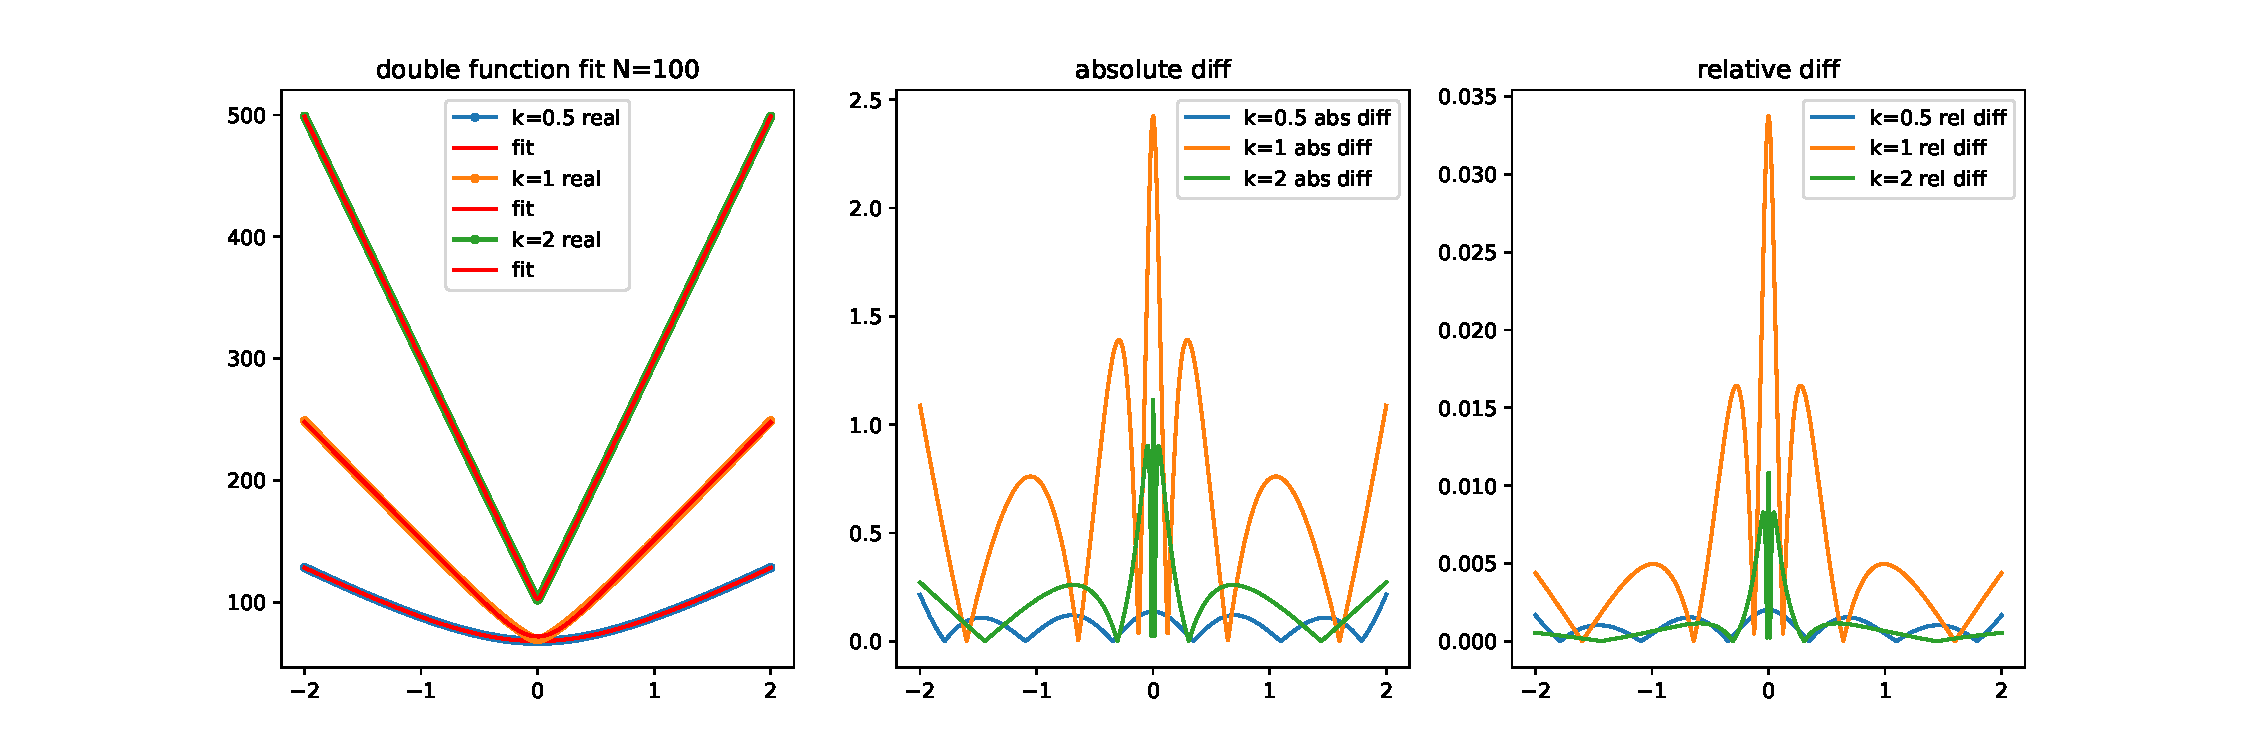
\includegraphics[width=1\textwidth]{img/CW_fit_N100.pdf}
    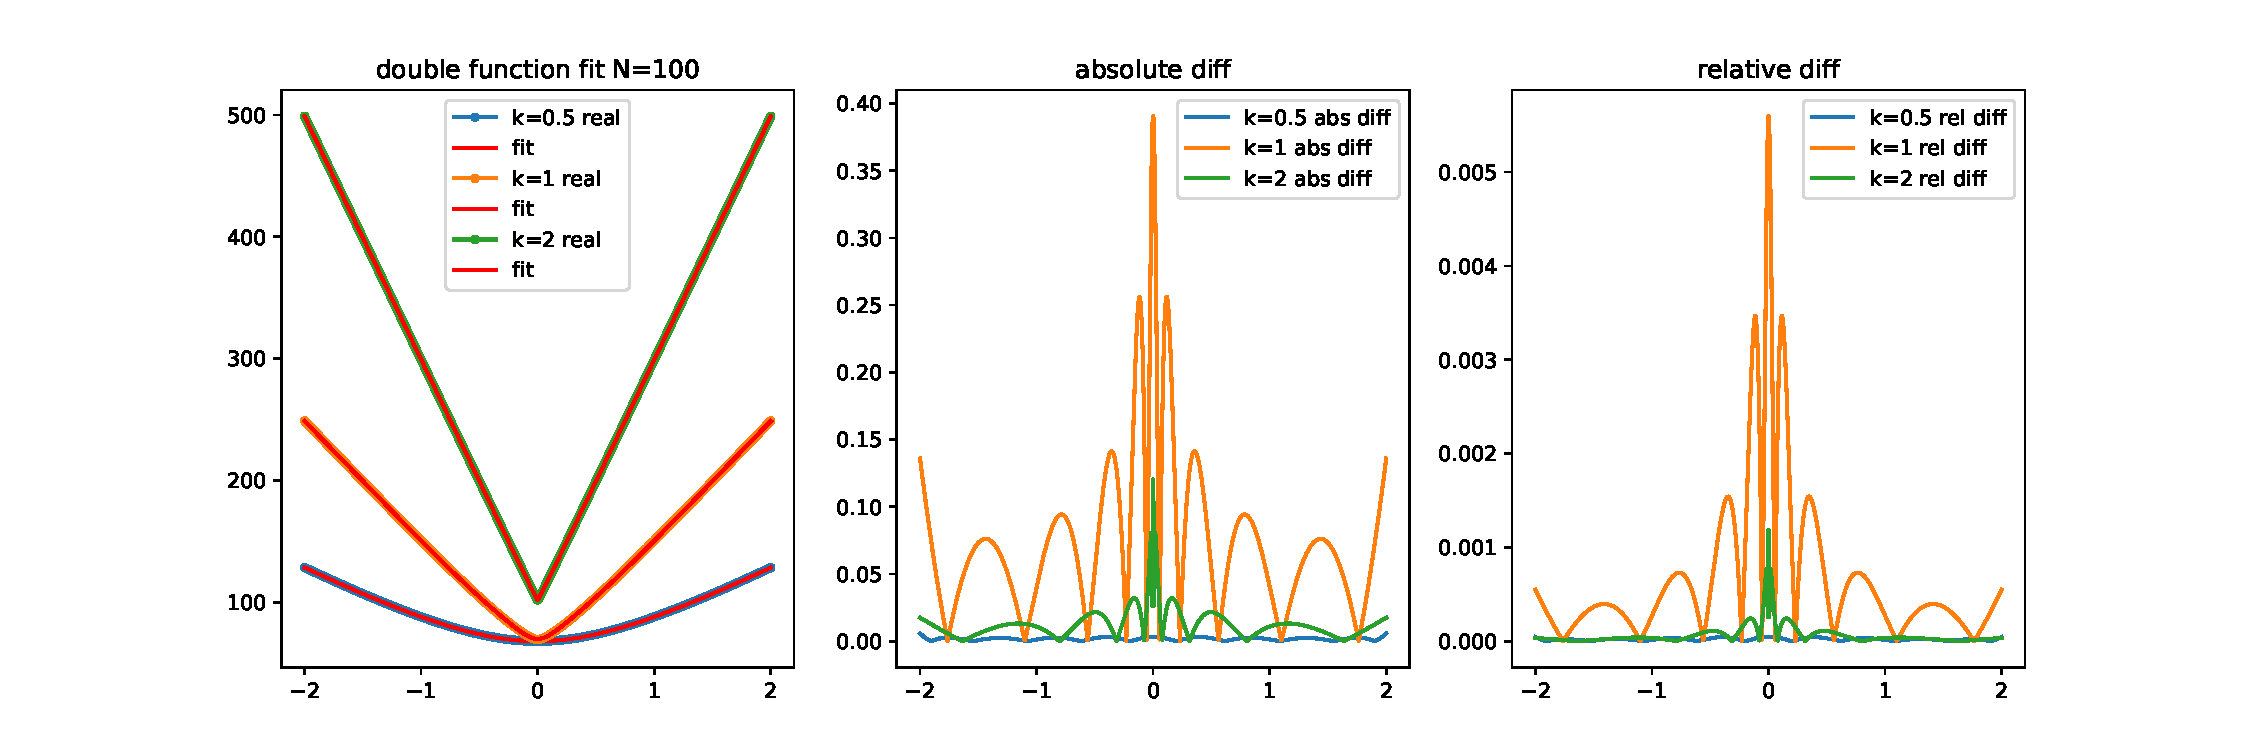
\includegraphics[width=1\textwidth]{img/CW_fit2_N100.pdf}
    \caption{Fit of eq.\ref{eq:CW_gauss_approx} at different values of $K=J\beta$. In the first row only one extreme is considered and two in the second row.}
    \label{fig:mesh1}
\end{figure}
The case of replica:
\[
 \int dt e^{-\frac{Nt^2}{2K}}\log\cosh(K*h+t) \approx \left(\sum_{t \in \text{Extrem}^+}  b_i^t + c_i^t\log\cosh(d_i^t+e_i^t h)\right)
\label{eq:CW_gauss_approx2}
\]

\begin{figure}[h]
    \centering
    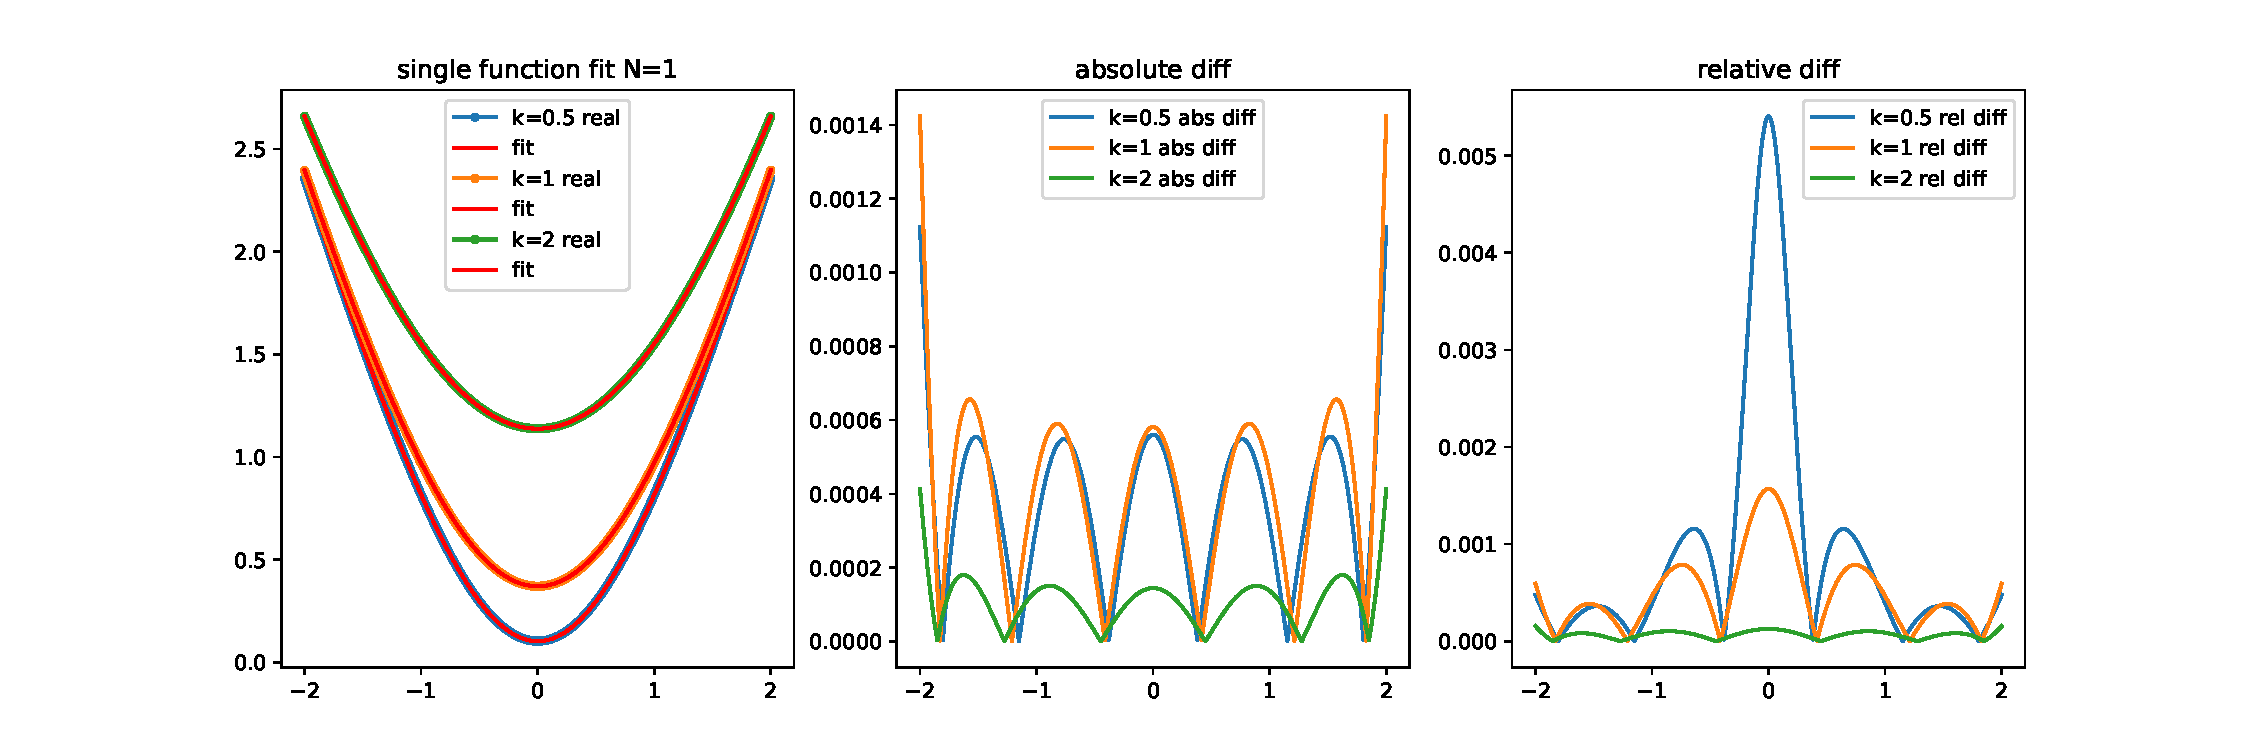
\includegraphics[width=1\textwidth]{img/RFIM_fit.pdf}
    \caption{Fit of eq.\ref{eq:CW_gauss_approx} at different values of $K=J\beta$. In the first row only one extreme is considered and two in the second row.}
    \label{fig:gauss_approx}
\end{figure}
\end{document}
